\documentclass[12pt,a4paper]{article}

% === PACKAGES ===
\usepackage[utf8]{inputenc}
\usepackage[T5]{fontenc}
\usepackage{amsmath, amssymb, graphicx, booktabs, geometry, hyperref, enumitem, float, caption, subcaption, algorithm, algpseudocode}

\geometry{right=2cm, left=3cm, top=2cm, bottom=2.5cm}
\renewcommand{\baselinestretch}{1.2}
\graphicspath{{figures/}}

% === MATH COMMANDS ===
\newcommand{\R}{\mathbb{R}}
\newcommand{\T}{\mathsf{T}}
\DeclareMathOperator{\diag}{diag}
\DeclareMathOperator{\rank}{rank}

% ================================================================
\begin{document}

\begin{center}
    {\Large\bfseries B\'{A}O C\'{A}O TI\H{E}N \DJ{}\d{O} LU\d{A}N V\u{A}N --- Ph\`{a}n 2} \\[8pt]
    {\large Critic-only ADP v\'{o}i Concurrent Learning \\
    Lo\d{a}i b\h{o} y\^{e}u c\`{a}u Persistence of Excitation} \\[14pt]
    \textbf{Nguy\~{e}n Th\`{a}nh Trung} \\[4pt]
    Chuy\^{e}n ng\`{a}nh: K\~{y} thu\d{a}t \DJ i\`{e}u khi\h{e}n v\`{a} T\d{u} \dj\d{o}ng h\'{o}a --- GVHD: PGS.TS. Nguy\~{e}n Ho\`{a}i Nam \\[2pt]
    \DJ\d{a}i h\d{o}c B\'{a}ch khoa H\`{a} N\d{o}i --- Th\'{a}ng 05/2026
\end{center}

\vspace{4pt}\hrule\vspace{8pt}

\noindent\textbf{C\^{o}ng vi\d{e}c \dj\~{a} ho\`{a}n th\`{a}nh:}
\begin{enumerate}[nosep]
    \item Nghi\^{e}n c\'{u}u l\'{y} thuy\'{e}t Critic-only ADP (gi\h{a}m t\`{u} 2 m\d{a}ng xu\'{o}ng 1 m\d{a}ng)
    \item Thi\'{e}t k\'{e} Concurrent Learning (CL): d\`{u}ng history stack thay t\'{i}n hi\d{e}u PE
    \item C\`{a}i \dj\d{a}t b\d{o} \dj i\`{e}u khi\h{e}n CL tr\^{e}n MATLAB, so s\'{a}nh v\'{o}i AC-ADP (SM1) v\`{a} Backstepping
    \item M\^{o} ph\h{o}ng tr\^{e}n 2 qu\~{y} \dj\d{a}o (tr\`{o}n, th\h{a}ng), ph\^{a}n t\'{i}ch h\d{o}i t\d{u} tr\d{o}ng s\'{o} v\`{a} sai s\'{o} Bellman
    \item K\'{e}t lu\d{a}n: CL \dj\d{a}t hi\d{e}u n\u{a}ng t\uhorn{}\ohorn{}ng \dj\uhorn{}\ohorn{}ng AC+PE m\`{a} \textbf{kh\^{o}ng c\`{a}n PE}
\end{enumerate}

% ================================================================
\section{\DJ\d{o}ng c\ohorn{} v\`{a} b\'{o}i c\h{a}nh}

\subsection{Nh\`{i}n l\d{a}i k\'{e}t qu\h{a} SM1 v\`{a} c\'{a}c h\d{a}n ch\'{e}}

Trong b\'{a}o c\'{a}o Seminar~1 (SM1), ch\'{u}ng t\^{o}i \dj\~{a} c\`{a}i \dj\d{a}t th\`{a}nh c\^{o}ng b\d{o} \dj i\`{e}u khi\h{e}n Actor-Critic ADP (Vamvoudakis \& Lewis, 2010) cho b\`{a}i to\'{a}n b\'{a}m qu\~{y} \dj\d{a}o robot di \dj\d{o}ng b\'{a}nh xe (WMR). Ph\uhorn{}\ohorn{}ng ph\'{a}p n\`{a}y s\h{u} d\d{u}ng hai m\d{a}ng n\ohorn{}-ron: m\d{a}ng Critic \dj\h{e} x\'{a}p x\h{i} h\`{a}m gi\'{a} tr\d{i} t\'{o}i \uhorn{}u, v\`{a} m\d{a}ng Actor \dj\h{e} x\'{a}p x\h{i} ch\'{i}nh s\'{a}ch \dj i\`{e}u khi\h{e}n t\'{o}i \uhorn{}u. K\'{e}t qu\h{a} cho th\'{a}y Actor-Critic ADP ho\d{a}t \dj\d{o}ng t\'{o}t tr\^{e}n qu\~{y} \dj\d{a}o \dj\uhorn{}\`{o}ng tr\`{o}n, tuy nhi\^{e}n b\d{o}c l\d{o} nhi\`{e}u h\d{a}n ch\'{e} khi \'{a}p d\d{u}ng tr\^{e}n qu\~{y} \dj\d{a}o \dj\uhorn{}\`{o}ng th\h{a}ng.

C\d{u} th\h{e}, b\'{o}n h\d{a}n ch\'{e} ch\'{i}nh \dj\~{a} \dj\uhorn{}\d{o}c x\'{a}c \dj\d{i}nh:

\begin{enumerate}
    \item \textbf{C\`{a}n kh\h{o}i t\d{a}o ``warm start'' (admissible initial policy):} N\'{e}u kh\h{o}i t\d{a}o tr\d{o}ng s\'{o} ban \dj\`{a}u $W_0 = 0$, h\d{e} th\'{o}ng m\'{a}t \h{o}n \dj\d{i}nh ngay l\d{a}p t\'{u}c. L\'{y} do l\`{a} khi $W_0 = 0$, ch\'{i}nh s\'{a}ch \dj i\`{e}u khi\h{e}n ban \dj\`{a}u $u_o = 0$ (kh\^{o}ng c\'{o} feedback), h\d{e} th\'{o}ng m\h{o} ho\d{a}t \dj\d{o}ng nh\uhorn{} kh\^{o}ng c\'{o} b\d{o} \dj i\`{e}u khi\h{e}n. Vi\d{e}c ch\d{o}n $W_0$ ph\`{u} h\d{o}p (\dj\h{a}m b\h{a}o ch\'{i}nh s\'{a}ch ban \dj\`{a}u \h{o}n \dj\d{i}nh) l\`{a} m\d{o}t y\^{e}u c\`{a}u kh\'{o} kh\u{a}n trong th\d{u}c t\'{e}.

    \item \textbf{T\'{i}n hi\d{e}u PE (Persistence of Excitation) ph\d{u} thu\d{o}c qu\~{y} \dj\d{a}o:} PE l\`{a} t\'{i}n hi\d{e}u nhi\~{e}u b\^{e}n ngo\`{a}i \dj\uhorn{}\d{o}c c\d{o}ng v\`{a}o l\d{e}nh \dj i\`{e}u khi\h{e}n nh\`{a}m ``k\'{i}ch th\'{i}ch'' h\d{e} th\'{o}ng, gi\'{u}p c\'{a}c tr\d{o}ng s\'{o} m\d{a}ng n\ohorn{}-ron h\d{o}i t\d{u}. Tr\^{e}n \dj\uhorn{}\`{o}ng tr\`{o}n ($\omega_r \neq 0$), b\h{a}n th\^{a}n qu\~{y} \dj\d{a}o \dj\~{a} c\'{o} s\d{u} k\'{i}ch th\'{i}ch t\d{u} nhi\^{e}n (v\d{a}n t\'{o}c g\'{o}c $\omega_r$ t\d{a}o coupling gi\~{u}a c\'{a}c tr\d{a}ng th\'{a}i), n\^{e}n PE c\d{o}ng th\^{e}m l\`{a} c\'{o} l\d{o}i. Tuy nhi\^{e}n, tr\^{e}n \dj\uhorn{}\`{o}ng th\h{a}ng ($\omega_r = 0$), PE tr\h{o} th\`{a}nh nhi\~{e}u thu\`{a}n t\'{u}y, ph\'{a} h\h{o}ng hi\d{e}u n\u{a}ng b\'{a}m qu\~{y} \dj\d{a}o.

    \item \textbf{Hai m\d{a}ng, nhi\`{e}u si\^{e}u tham s\'{o}:} V\'{o}i c\'{a}c tham s\'{o} $\alpha_c$, $\alpha_{a1}$, $\alpha_{a2}$, $\kappa_c$, c\`{u}ng v\'{o}i bi\^{e}n \dj\d{o}, t\`{a}n s\'{o} PE --- vi\d{e}c tinh ch\h{i}nh (tuning) ho\`{a}n to\`{a}n b\`{a}ng tay v\`{a} r\'{a}t nh\d{a}y c\h{a}m v\'{o}i \dj i\`{e}u ki\d{e}n v\d{a}n h\`{a}nh.

    \item \textbf{H\d{o}i t\d{u} ch\d{a}m tr\^{e}n \dj\uhorn{}\`{o}ng th\h{a}ng:} $z_\text{rms} = 0.36$\,m (trung b\`{i}nh b\`{i}nh ph\uhorn{}\ohorn{}ng c\h{u}a sai l\d{e}ch) sau 120\,s v\~{a}n c\`{o}n r\'{a}t l\'{o}n, cho th\'{a}y tr\d{o}ng s\'{o} ch\uhorn{}a h\d{o}i t\d{u} \dj\'{e}n nghi\d{e}m t\'{o}i \uhorn{}u.
\end{enumerate}

\subsection{M\d{u}c ti\^{e}u c\h{u}a SM2}

T\`{u} nh\~{u}ng h\d{a}n ch\'{e} n\^{e}u tr\^{e}n, m\d{u}c ti\^{e}u c\h{u}a Seminar~2 \dj\uhorn{}\d{o}c x\'{a}c \dj\d{i}nh r\~{o} r\`{a}ng:
\begin{itemize}
    \item \textbf{Gi\h{a}m t\`{u} 2 m\d{a}ng xu\'{o}ng 1 m\d{a}ng} (Critic-only): lo\d{a}i b\h{o} m\d{a}ng Actor, suy ch\'{i}nh s\'{a}ch tr\d{u}c ti\'{e}p t\`{u} m\d{a}ng Critic duy nh\'{a}t.
    \item \textbf{Lo\d{a}i b\h{o} ho\`{a}n to\`{a}n y\^{e}u c\`{a}u PE} b\`{a}ng k\~{y} thu\d{a}t Concurrent Learning (CL): s\h{u} d\d{u}ng d\~{u} li\d{e}u l\d{i}ch s\h{u} thay v\`{i} t\'{i}n hi\d{e}u k\'{i}ch th\'{i}ch b\^{e}n ngo\`{a}i.
\end{itemize}

N\'{e}u th\`{a}nh c\^{o}ng, b\d{o} \dj i\`{e}u khi\h{e}n m\'{o}i s\~{e} \dj\ohorn{}n gi\h{a}n h\ohorn{}n (1 m\d{a}ng, \'{i}t si\^{e}u tham s\'{o}), \dj\'{o}ng th\`{o}i ho\d{a}t \dj\d{o}ng t\'{o}t tr\^{e}n m\d{o}i lo\d{a}i qu\~{y} \dj\d{a}o m\`{a} kh\^{o}ng ph\d{u} thu\d{o}c v\`{a}o \dj i\`{e}u ki\d{e}n PE.

% ================================================================
\section{L\'{y} thuy\'{e}t: Critic-only ADP}

\subsection{T\`{u} hai m\d{a}ng sang m\d{o}t m\d{a}ng}

Nh\uhorn{} \dj\~{a} tr\`{i}nh b\`{a}y trong SM1, ki\'{e}n tr\'{u}c Actor-Critic ADP s\h{u} d\d{u}ng hai m\d{a}ng n\ohorn{}-ron ri\^{e}ng bi\d{e}t:

\begin{itemize}
    \item \textbf{M\d{a}ng Critic} x\'{a}p x\h{i} h\`{a}m gi\'{a} tr\d{i} (value function):
    \begin{equation}
        \hat{V}(z) = \hat{W}_c^\T \phi(z)
    \end{equation}
    trong \dj\'{o} $\hat{W}_c \in \R^l$ l\`{a} vector tr\d{o}ng s\'{o} Critic, $\phi(z) \in \R^l$ l\`{a} vector h\`{a}m c\ohorn{} s\h{o} (basis function). H\`{a}m gi\'{a} tr\d{i} $\hat{V}(z)$ \dj\'{a}nh gi\'{a} ``chi ph\'{i} t\uhorn{}\ohorn{}ng lai'' c\h{u}a vi\d{e}c \h{o} tr\d{a}ng th\'{a}i $z$ hi\d{e}n t\d{a}i.

    \item \textbf{M\d{a}ng Actor} x\'{a}p x\h{i} ch\'{i}nh s\'{a}ch \dj i\`{e}u khi\h{e}n t\'{o}i \uhorn{}u:
    \begin{equation}
        \hat{u}_o = -\frac{1}{2} R^{-1}\, g(z)^\T\, \nabla\phi^\T\, \hat{W}_a
    \end{equation}
    trong \dj\'{o} $\hat{W}_a \in \R^l$ l\`{a} vector tr\d{o}ng s\'{o} Actor, $g(z)$ l\`{a} ma tr\d{a}n \dj\`{a}u v\`{a}o c\h{u}a h\d{e} th\'{o}ng, $\nabla\phi = \partial\phi/\partial z$ l\`{a} Jacobian c\h{u}a h\`{a}m c\ohorn{} s\h{o}.
\end{itemize}

M\d{u}c \dj\'{i}ch c\h{u}a qu\'{a} tr\`{i}nh h\d{o}c l\`{a} c\h{a} hai vector tr\d{o}ng s\'{o} \dj\`{e}u h\d{o}i t\d{u} v\`{e} gi\'{a} tr\d{i} t\'{o}i \uhorn{}u:
\begin{equation}
    \hat{W}_a \to \hat{W}_c \to W^*
\end{equation}
\'{Y} ngh\~{i}a v\d{a}t l\'{y}: khi qu\'{a} tr\`{i}nh h\d{o}c k\'{e}t th\'{u}c, tr\d{o}ng s\'{o} Actor v\`{a} Critic \dj\`{e}u x\'{a}p x\h{i} c\`{u}ng m\d{o}t gi\'{a} tr\d{i} $W^*$ --- nghi\d{e}m c\h{u}a ph\uhorn{}\ohorn{}ng tr\`{i}nh Hamilton-Jacobi-Bellman (HJB). M\d{o}t c\^{a}u h\h{o}i t\d{u} nhi\^{e}n \dj\d{a}t ra: \textit{n\'{e}u cu\'{o}i c\`{u}ng $\hat{W}_a \approx \hat{W}_c$, t\d{a}i sao kh\^{o}ng d\`{u}ng tr\d{u}c ti\'{e}p $\hat{W}_c$ \dj\h{e} t\'{i}nh ch\'{i}nh s\'{a}ch \dj i\`{e}u khi\h{e}n?}

\textbf{C\'{a}ch ti\'{e}p c\d{a}n Critic-only:} Lo\d{a}i b\h{o} ho\`{a}n to\`{a}n m\d{a}ng Actor, suy ch\'{i}nh s\'{a}ch \dj i\`{e}u khi\h{e}n tr\d{u}c ti\'{e}p t\`{u} m\d{a}ng Critic:
\begin{equation}\label{eq:cl_control}
    \boxed{u_o = -\frac{1}{2} R^{-1}\, g(z)^\T\, \nabla\phi^\T\, W}
\end{equation}
trong \dj\'{o} $W \in \R^l$ l\`{a} vector tr\d{o}ng s\'{o} Critic \textit{duy nh\'{a}t}. S\'{o} tham s\'{o} c\`{a}n h\d{o}c gi\h{a}m t\`{u} $2l = 12$ (6 Critic + 6 Actor) xu\'{o}ng c\`{o}n $l = 6$.

\textbf{\Uhorn{}u \dj i\h{e}m c\h{u}a Critic-only so v\'{o}i Actor-Critic:}
\begin{itemize}
    \item \textbf{\'{I}t tham s\'{o} h\d{o}c h\ohorn{}n:} Ch\h{i} c\`{o}n 6 tr\d{o}ng s\'{o} thay v\`{i} 12, gi\h{a}m \dj\d{o} ph\'{u}c t\d{a}p t\'{i}nh to\'{a}n v\`{a} t\u{a}ng t\'{i}nh \h{o}n \dj\d{i}nh c\h{u}a qu\'{a} tr\`{i}nh h\d{o}c.
    \item \textbf{Lo\d{a}i b\h{o} lu\d{a}t c\d{a}p nh\d{a}t Actor:} Kh\^{o}ng c\`{o}n c\'{a}c si\^{e}u tham s\'{o} $\alpha_{a1}$, $\alpha_{a2}$ c\h{u}a Actor update, gi\h{a}m kh\'{o} kh\u{a}n khi tuning.
    \item \textbf{Ch\'{i}nh s\'{a}ch thay \dj\h{o}i ``m\uhorn{}\d{o}t'':} V\`{i} $u_o$ \dj\uhorn{}\d{o}c t\'{i}nh tr\d{u}c ti\'{e}p t\`{u} $W$, kh\^{o}ng c\'{o} \dj\d{o} tr\~{e} gi\~{u}a Critic v\`{a} Actor nh\uhorn{} trong ki\'{e}n tr\'{u}c hai m\d{a}ng. \DJ i\`{e}u n\`{a}y gi\'{u}p ch\'{i}nh s\'{a}ch \dj i\`{e}u khi\h{e}n bi\'{e}n \dj\h{o}i li\^{e}n t\d{u}c v\`{a} tr\ohorn{}n h\ohorn{}n theo th\`{o}i gian.
\end{itemize}

\textbf{V\'{a}n \dj\`{e} m\'{o}i ph\'{a}t sinh:} M\d{a}c d\`{u} \dj\ohorn{}n gi\h{a}n h\ohorn{}n v\`{e} c\'{a}u tr\'{u}c, Critic-only v\~{a}n g\d{a}p ph\h{a}i v\'{a}n \dj\`{e} c\ohorn{} b\h{a}n: n\'{e}u ch\h{i} s\h{u} d\d{u}ng online gradient descent (c\d{a}p nh\d{a}t tr\d{o}ng s\'{o} d\d{u}a tr\^{e}n d\~{u} li\d{e}u hi\d{e}n t\d{a}i), h\d{e} th\'{o}ng v\~{a}n c\`{a}n \dj i\`{e}u ki\d{e}n PE \dj\h{e} \dj\h{a}m b\h{a}o h\d{o}i t\d{u}. \DJ\^{a}y ch\'{i}nh l\`{a} l\'{y} do c\`{a}n k\'{e}t h\d{o}p v\'{o}i \textbf{Concurrent Learning}.

\subsection{Sai s\'{o} Bellman v\`{a} c\d{a}p nh\d{a}t online}

\DJ\h{e} hi\h{e}u c\ohorn{} ch\'{e} h\d{o}c c\h{u}a Critic-only, ta c\`{a}n \dj\d{i}nh ngh\~{i}a sai s\'{o} Bellman --- th\uhorn{}\'{o}c \dj o ``kho\h{a}ng c\'{a}ch'' gi\~{u}a ch\'{i}nh s\'{a}ch hi\d{e}n t\d{a}i v\`{a} ch\'{i}nh s\'{a}ch t\'{o}i \uhorn{}u.

Tr\uhorn{}\'{o}c h\'{e}t, \dj\d{i}nh ngh\~{i}a vector \dj\d{a}o h\`{a}m c\ohorn{} s\h{o} theo \dj\d{o}ng h\d{o}c:
\begin{equation}
    \sigma = \nabla\phi\,(f + g\, u_o) \in \R^6
\end{equation}
\'{Y} ngh\~{i}a v\d{a}t l\'{y}: $\sigma$ l\`{a} t\'{o}c \dj\d{o} thay \dj\h{o}i c\h{u}a h\`{a}m c\ohorn{} s\h{o} $\phi(z)$ theo th\`{o}i gian, \dj\d{o}c theo qu\~{y} \dj\d{a}o c\h{u}a h\d{e} th\'{o}ng khi \'{a}p d\d{u}ng ch\'{i}nh s\'{a}ch $u_o$. N\'{o} ph\h{a}n \'{a}nh c\'{a}ch h\d{e} th\'{o}ng ``di chuy\h{e}n'' trong kh\^{o}ng gian tr\d{a}ng th\'{a}i.

Sai s\'{o} Bellman \dj\uhorn{}\d{o}c \dj\d{i}nh ngh\~{i}a:
\begin{equation}\label{eq:bellman}
    \delta = W^\T \sigma + z^\T Q\, z + u_o^\T R\, u_o
\end{equation}
\'{Y} ngh\~{i}a: $\delta$ \dj o l\uhorn{}\`{o}ng m\'{u}c \dj\d{o} vi ph\d{a}m ph\uhorn{}\ohorn{}ng tr\`{i}nh HJB. Khi $W = W^*$ (nghi\d{e}m t\'{o}i \uhorn{}u), $\delta = 0$. Do \dj\'{o}, m\d{u}c ti\^{e}u c\h{u}a qu\'{a} tr\`{i}nh h\d{o}c l\`{a} \dj i\`{e}u ch\h{i}nh $W$ sao cho $\delta \to 0$.

Th\`{a}nh ph\`{a}n $z^\T Q z$ \dj\d{a}i di\d{e}n cho chi ph\'{i} sai l\d{e}ch tr\d{a}ng th\'{a}i (c\`{a}ng l\'{o}n khi robot \dj i l\d{e}ch qu\~{y} \dj\d{a}o), v\`{a} $u_o^\T R u_o$ \dj\d{a}i di\d{e}n cho chi ph\'{i} n\u{a}ng l\uhorn{}\d{o}ng \dj i\`{e}u khi\h{e}n (c\`{a}ng l\'{o}n khi l\d{e}nh \dj i\`{e}u khi\h{e}n c\`{a}ng m\d{a}nh).

Lu\d{a}t c\d{a}p nh\d{a}t online (gradient descent):
\begin{equation}\label{eq:online_update}
    \dot{W}_\text{online} = -\alpha\, \bar{\sigma}\, \delta, \quad \bar{\sigma} = \frac{\sigma}{(1+\sigma^\T\sigma)^2}
\end{equation}
trong \dj\'{o} $\alpha > 0$ l\`{a} t\'{o}c \dj\d{o} h\d{o}c (learning rate), $\bar{\sigma}$ l\`{a} phi\^{e}n b\h{a}n chu\h{a}n h\'{o}a c\h{u}a $\sigma$ (tr\'{a}nh ph\'{a}t t\'{a}n s\'{o} khi $\|\sigma\|$ l\'{o}n).

\textbf{H\d{a}n ch\'{e} c\h{u}a c\d{a}p nh\d{a}t online thu\`{a}n t\'{u}y:} T\d{a}i m\~{o}i th\`{o}i \dj i\h{e}m, ch\h{i} c\'{o} \textit{duy nh\'{a}t m\d{o}t h\uhorn{}\'{o}ng} $\bar{\sigma}$ \dj\uhorn{}\d{o}c s\h{u} d\d{u}ng \dj\h{e} c\d{a}p nh\d{a}t $W$. Trong kh\^{o}ng gian $\R^6$, c\`{a}n \'{i}t nh\'{a}t 6 h\uhorn{}\'{o}ng \dj\d{o}c l\d{a}p tuy\'{e}n t\'{i}nh \dj\h{e} x\'{a}c \dj\d{i}nh \dj\`{a}y \dj\h{u} $W^*$. \DJ i\`{e}u n\`{a}y \dj\`{o}i h\h{o}i PE --- t\'{i}n hi\d{e}u b\^{e}n ngo\`{a}i ``k\'{i}ch th\'{i}ch'' $\sigma$ quay qua nhi\`{e}u h\uhorn{}\'{o}ng kh\'{a}c nhau. Kh\^{o}ng c\'{o} PE, h\d{o}c ch\d{a}m v\`{a} c\'{o} th\h{e} kh\^{o}ng h\d{o}i t\d{u}.

% ================================================================
\section{Concurrent Learning --- Thay th\'{e} PE}

\subsection{\'{Y} t\uhorn{}\h{o}ng ch\'{i}nh}

Concurrent Learning (CL), \dj\`{e} xu\'{a}t b\h{o}i Chowdhary \& Johnson (2010), gi\h{a}i quy\'{e}t v\'{a}n \dj\`{e} PE b\`{a}ng m\d{o}t \'{y} t\uhorn{}\h{o}ng \dj\ohorn{}n gi\h{a}n nh\uhorn{}ng hi\d{e}u qu\h{a}: \textit{thay v\`{i} ch\h{i} d\`{u}ng d\~{u} li\d{e}u hi\d{e}n t\d{a}i, h\~{a}y l\uhorn{}u l\d{a}i v\`{a} t\'{a}i s\h{u} d\d{u}ng d\~{u} li\d{e}u c\~{u}}.

C\d{u} th\h{e}, ta x\^{a}y d\d{u}ng m\d{o}t \textit{history stack} (b\d{o} nh\'{o} l\d{i}ch s\h{u}):
\begin{equation}
    \mathcal{H} = \big\{ (\sigma_j, c_j) \big\}_{j=1}^{N_H}
\end{equation}
trong \dj\'{o}:
\begin{itemize}[nosep]
    \item $\sigma_j = \nabla\phi(z_j)\,(f(z_j) + g(z_j)\,u_{o,j})$: vector \dj\d{a}o h\`{a}m c\ohorn{} s\h{o} t\d{a}i th\`{o}i \dj i\h{e}m $t_j$
    \item $c_j = z_j^\T Q\, z_j + u_{o,j}^\T R\, u_{o,j}$: chi ph\'{i} t\'{u}c th\`{o}i t\d{a}i $t_j$
\end{itemize}

M\~{o}i c\d{a}p $(\sigma_j, c_j)$ \dj\uhorn{}\d{o}c ghi nh\d{a}n \dj\d{i}nh k\`{y} (m\~{o}i 50\,ms) trong su\'{o}t qu\'{a} tr\`{i}nh v\d{a}n h\`{a}nh. \'{Y} ngh\~{i}a v\d{a}t l\'{y}: \dj\^{a}y l\`{a} ``kinh nghi\d{e}m'' c\h{u}a h\d{e} th\'{o}ng --- m\~{o}i \dj i\h{e}m d\~{u} li\d{e}u ghi l\d{a}i m\d{o}t ``kho\h{a}nh kh\'{a}c'' c\h{u}a qu\'{a} tr\`{i}nh v\d{a}n h\`{a}nh, bao g\`{o}m c\h{a} h\uhorn{}\'{o}ng chuy\h{e}n \dj\d{o}ng ($\sigma_j$) v\`{a} chi ph\'{i} ($c_j$).

T\d{a}i m\~{o}i b\uhorn{}\'{o}c c\d{a}p nh\d{a}t, ta t\'{i}nh \textbf{sai s\'{o} Bellman cho t\`{u}ng \dj i\h{e}m l\d{i}ch s\h{u}} s\h{u} d\d{u}ng tr\d{o}ng s\'{o} $W$ hi\d{e}n t\d{a}i:
\begin{equation}\label{eq:delta_hist}
    \delta_j = W^\T \sigma_j + c_j, \quad j = 1, \ldots, N_H
\end{equation}
\'{Y} ngh\~{i}a: v\'{o}i tr\d{o}ng s\'{o} $W$ hi\d{e}n t\d{a}i, n\'{e}u quay l\d{a}i th\`{o}i \dj i\h{e}m $t_j$, sai s\'{o} Bellman s\~{e} l\`{a} bao nhi\^{e}u? \DJ\^{a}y l\`{a} c\'{a}ch ``h\h{o}i l\d{a}i kinh nghi\d{e}m c\~{u}'' v\'{o}i ``ki\'{e}n th\'{u}c m\'{o}i''.

Lu\d{a}t c\d{a}p nh\d{a}t CL:
\begin{equation}\label{eq:cl_update}
    \dot{W}_\text{CL} = -\frac{\alpha_h}{N_H} \sum_{j=1}^{N_H} \bar{\sigma}_j\, \delta_j
\end{equation}
trong \dj\'{o} $\alpha_h > 0$ l\`{a} t\'{o}c \dj\d{o} h\d{o}c t\`{u} d\~{u} li\d{e}u l\d{i}ch s\h{u}, $\bar{\sigma}_j = \sigma_j / (1 + \sigma_j^\T \sigma_j)^2$ l\`{a} phi\^{e}n b\h{a}n chu\h{a}n h\'{o}a.

\textbf{T\d{a}i sao CL thay th\'{e} \dj\uhorn{}\d{o}c PE?} M\~{o}i \dj i\h{e}m l\d{i}ch s\h{u} $\sigma_j$ \dj\uhorn{}\d{o}c ghi t\d{a}i c\'{a}c th\`{o}i \dj i\h{e}m kh\'{a}c nhau, khi tr\d{a}ng th\'{a}i $z_j$ kh\'{a}c nhau, n\^{e}n c\'{a}c h\uhorn{}\'{o}ng $\sigma_j$ c\~{u}ng kh\'{a}c nhau. T\h{o}ng $\sum \bar{\sigma}_j \delta_j$ t\uhorn{}\ohorn{}ng \dj\uhorn{}\ohorn{}ng m\d{o}t ``t\'{i}ch ph\^{a}n'' tr\^{e}n nhi\`{e}u h\uhorn{}\'{o}ng trong $\R^6$, cung c\'{a}p \dj\h{u} th\^{o}ng tin \dj\h{e} x\'{a}c \dj\d{i}nh $W^*$ m\`{a} \textit{kh\^{o}ng c\`{a}n th\^{e}m nhi\~{e}u k\'{i}ch th\'{i}ch b\^{e}n ngo\`{a}i}.

\subsection{\DJ i\`{e}u ki\d{e}n rank (thay th\'{e} PE)}

Trong l\'{y} thuy\'{e}t Actor-Critic truy\`{e}n th\'{o}ng, \dj i\`{e}u ki\d{e}n PE y\^{e}u c\`{a}u t\'{i}n hi\d{e}u $\sigma(t)$ ph\h{a}i ``qu\'{e}t'' qua \dj\h{u} m\d{o}i h\uhorn{}\'{o}ng trong $\R^l$ trong m\d{o}t kho\h{a}ng th\`{o}i gian. \DJ\^{a}y l\`{a} \dj i\`{e}u ki\d{e}n kh\'{o} ki\h{e}m tra v\`{a} ph\d{u} thu\d{o}c v\`{a}o qu\~{y} \dj\d{a}o tham chi\'{e}u.

V\'{o}i Concurrent Learning, \dj i\`{e}u ki\d{e}n PE \dj\uhorn{}\d{o}c thay th\'{e} b\h{o}i \dj i\`{e}u ki\d{e}n rank \dj\ohorn{}n gi\h{a}n h\ohorn{}n nhi\`{e}u:
\begin{equation}\label{eq:rank_cond}
    \rank\big(\Sigma\big) = l, \quad \Sigma = [\sigma_1, \sigma_2, \ldots, \sigma_{N_H}] \in \R^{l \times N_H}
\end{equation}
\'{Y} ngh\~{i}a: ma tr\d{a}n $\Sigma$ (g\h{o}m c\'{a}c vector $\sigma_j$ x\'{e}p th\`{a}nh c\d{o}t) c\`{a}n c\'{o} h\d{a}ng \dj\`{a}y \dj\h{u}, t\'{u}c l\`{a} c\'{a}c \dj i\h{e}m d\~{u} li\d{e}u trong history stack ph\h{a}i ``\dj\h{u} \dj a d\d{a}ng'' v\`{e} h\uhorn{}\'{o}ng.

V\'{o}i $l = 6$ (s\'{o} tr\d{o}ng s\'{o} c\`{a}n h\d{o}c), ch\h{i} c\`{a}n $N_H \geq 6$ \dj i\h{e}m d\~{u} li\d{e}u \dj\d{o}c l\d{a}p tuy\'{e}n t\'{i}nh. Trong th\d{u}c t\'{e}, v\'{o}i $N_H = 200$ \dj i\h{e}m v\`{a} ghi m\~{o}i 50\,ms, \dj i\`{e}u ki\d{e}n rank \dj\uhorn{}\d{o}c th\h{o}a m\~{a}n d\~{e} d\`{a}ng ch\h{i} sau v\`{a}i gi\^{a}y v\d{a}n h\`{a}nh (khi robot c\`{o}n \dj ang b\'{a}m v\`{e} qu\~{y} \dj\d{a}o, tr\d{a}ng th\'{a}i thay \dj\h{o}i nhanh, t\d{a}o ra c\'{a}c $\sigma_j$ \dj a d\d{a}ng).

So v\'{o}i PE, \dj i\`{e}u ki\d{e}n rank c\'{o} hai \uhorn{}u \dj i\h{e}m l\'{o}n:
\begin{enumerate}[nosep]
    \item \textbf{D\~{e} ki\h{e}m tra:} Ch\h{i} c\`{a}n t\'{i}nh rank c\h{u}a ma tr\d{a}n $\Sigma$ (m\d{o}t ph\'{e}p to\'{a}n \dj\ohorn{}n gi\h{a}n), thay v\`{i} ki\h{e}m tra t\'{i}ch ph\^{a}n t\'{i}n hi\d{e}u theo th\`{o}i gian.
    \item \textbf{Kh\^{o}ng ph\d{u} thu\d{o}c qu\~{y} \dj\d{a}o:} M\d{o}i qu\~{y} \dj\d{a}o (\dj\uhorn{}\`{o}ng tr\`{o}n, \dj\uhorn{}\`{o}ng th\h{a}ng, hay b\'{a}t k\`{y}) \dj\`{e}u t\d{a}o ra d\~{u} li\d{e}u \dj\h{u} \dj a d\d{a}ng trong giai \dj o\d{a}n \dj\`{a}u (khi sai l\d{e}ch c\`{o}n l\'{o}n).
\end{enumerate}

\subsection{T\h{o}ng h\d{o}p c\d{a}p nh\d{a}t tr\d{o}ng s\'{o}}

K\'{e}t h\d{o}p c\h{a} ba th\`{a}nh ph\`{a}n, lu\d{a}t c\d{a}p nh\d{a}t tr\d{o}ng s\'{o} \dj\`{a}y \dj\h{u} l\`{a}:
\begin{equation}\label{eq:total_update}
    \boxed{\dot{W} = \underbrace{-\alpha\, \bar{\sigma}\, \delta}_\text{online} \; \underbrace{-\frac{\alpha_h}{N_H} \sum_j \bar{\sigma}_j\, \delta_j}_\text{Concurrent Learning} \; \underbrace{-\kappa\, W}_\text{$\sigma$-modification}}
\end{equation}

Ba th\`{a}nh ph\`{a}n v\`{a} vai tr\`{o} c\h{u}a ch\'{u}ng:
\begin{enumerate}
    \item \textbf{Online gradient} ($\alpha = 0.5$): C\d{a}p nh\d{a}t t\'{u}c th\`{o}i t\`{u} d\~{u} li\d{e}u hi\d{e}n t\d{a}i. Th\`{a}nh ph\`{a}n n\`{a}y ph\h{a}n \'{u}ng nhanh v\'{o}i thay \dj\h{o}i c\h{u}a h\d{e} th\'{o}ng, nh\uhorn{}ng ch\h{i} cung c\'{a}p th\^{o}ng tin theo m\d{o}t h\uhorn{}\'{o}ng $\bar{\sigma}$.

    \item \textbf{Concurrent Learning gradient} ($\alpha_h = 0.5$): C\d{a}p nh\d{a}t t\`{u} d\~{u} li\d{e}u l\d{i}ch s\h{u} (``kinh nghi\d{e}m''). Th\`{a}nh ph\`{a}n n\`{a}y cung c\'{a}p th\^{o}ng tin theo nhi\`{e}u h\uhorn{}\'{o}ng $\bar{\sigma}_j$ kh\'{a}c nhau, b\`{u} \dj\'{a}p cho s\d{u} thi\'{e}u th\^{o}ng tin c\h{u}a online gradient.

    \item \textbf{$\sigma$-modification} ($\kappa = 0.01$): Th\`{a}nh ph\`{a}n weight decay, k\'{e}o $W$ v\`{e} g\`{a}n g\'{o}c t\d{o}a \dj\d{o}. Vai tr\`{o}: ch\'{o}ng ph\'{a}t t\'{a}n tr\d{o}ng s\'{o} (weight drift) khi d\~{u} li\d{e}u nhi\~{e}u ho\d{a}c m\^{o} h\`{i}nh kh\^{o}ng ch\'{i}nh x\'{a}c.
\end{enumerate}

\subsection{C\`{a}i \dj\d{a}t vectorized trong MATLAB}

Trong MATLAB, vi\d{e}c d\`{u}ng v\`{o}ng l\d{a}p \texttt{for} tr\^{e}n $N_H = 200$ \dj i\h{e}m l\`{a} ch\d{a}m do MATLAB l\`{a} ng\^{o}n ng\~{u} thong d\d{i}ch. Gi\h{a}i ph\'{a}p l\`{a} vectorize --- bi\'{e}n \dj\h{o}i c\'{a}c ph\'{e}p t\'{i}nh th\`{a}nh ph\'{e}p to\'{a}n ma tr\d{a}n:

G\d{o}i $S = [\sigma_1, \ldots, \sigma_{N_H}] \in \R^{6 \times N_H}$ v\`{a} $C = [c_1, \ldots, c_{N_H}] \in \R^{1 \times N_H}$, ta c\'{o}:
\begin{align}
    \Delta &= W^\T S + C \in \R^{1 \times N_H} & &\text{(Bellman error cho to\`{a}n b\d{o} history)} \\
    \bar{S} &= S \oslash \big(1 + \|S_{\cdot,j}\|^2\big)^2 \in \R^{6 \times N_H} & &\text{(chu\h{a}n h\'{o}a theo c\d{o}t)} \\
    \dot{W}_\text{CL} &= -\frac{\alpha_h}{N_H}\, \bar{S}\, \Delta^\T & &\text{(t\'{i}ch ma tr\d{a}n duy nh\'{a}t)}
\end{align}
trong \dj\'{o} ph\'{e}p chia $\oslash$ th\d{u}c hi\d{e}n theo c\d{o}t (element-wise division). To\`{a}n b\d{o} vi\d{e}c t\'{i}nh CL gradient quy v\`{e} m\d{o}t ph\'{e}p nh\^{a}n ma tr\d{a}n $\R^{6 \times N_H} \times \R^{N_H \times 1}$, nhanh h\ohorn{}n v\`{o}ng \texttt{for} kho\h{a}ng $100\times$ trong MATLAB.

% ================================================================
\section{Thi\'{e}t l\d{a}p m\^{o} ph\h{o}ng}

\subsection{C\'{a}u h\`{i}nh chung}

M\^{o} ph\h{o}ng \dj\uhorn{}\d{o}c th\d{u}c hi\d{e}n tr\^{e}n MATLAB R2023a v\'{o}i c\'{a}c thi\'{e}t l\d{a}p sau:

\begin{itemize}
    \item \textbf{M\^{o} h\`{i}nh:} Kinematic-only (ch\h{i} v\`{o}ng ngo\`{a}i \dj\d{o}ng h\d{o}c, kh\^{o}ng x\'{e}t v\`{o}ng trong \dj\d{o}ng l\d{u}c h\d{o}c). M\^{o} h\`{i}nh sai l\d{e}ch b\'{a}m qu\~{y} \dj\d{a}o:
    \begin{equation}
        \dot{z} = f(z) + g(z)\,(u_r + u_o)
    \end{equation}
    v\'{o}i $z = [z_x, z_y, z_\theta]^\T$ l\`{a} sai l\d{e}ch v\d{i} tr\'{i}/g\'{o}c, $u_r$ l\`{a} l\d{e}nh feedforward, $u_o$ l\`{a} l\d{e}nh feedback t\'{o}i \uhorn{}u.

    \item \textbf{Ph\uhorn{}\ohorn{}ng ph\'{a}p t\'{i}ch ph\^{a}n:} Euler hi\d{e}n (explicit), b\uhorn{}\'{o}c th\`{o}i gian $\Delta t = 0.001$\,s, t\h{o}ng th\`{o}i gian m\^{o} ph\h{o}ng $T = 120$\,s ($120{,}000$ b\uhorn{}\'{o}c).

    \item \textbf{Sai l\d{e}ch ban \dj\`{a}u:} $z_0 = q_0 - q_{r,0} = [0.2,\; -0.1,\; 0.1]$ (m, m, rad). \'{Y} ngh\~{i}a: robot b\'{a}t \dj\`{a}u l\d{e}ch 20\,cm theo ph\uhorn{}\ohorn{}ng $x$, l\d{e}ch $-10$\,cm theo ph\uhorn{}\ohorn{}ng $y$, v\`{a} l\d{e}ch 0.1\,rad ($\approx 5.7^\circ$) v\`{e} h\uhorn{}\'{o}ng.

    \item \textbf{Qu\~{y} \dj\d{a}o tham chi\'{e}u:}
    \begin{itemize}[nosep]
        \item \DJ\uhorn{}\`{o}ng tr\`{o}n: b\'{a}n k\'{i}nh $R = 2$\,m, v\d{a}n t\'{o}c d\`{a}i $v_r = 0.3$\,m/s, v\d{a}n t\'{o}c g\'{o}c $\omega_r = v_r/R = 0.15$\,rad/s.
        \item \DJ\uhorn{}\`{o}ng th\h{a}ng: $v_r = 0.3$\,m/s, $\omega_r = 0$ (kh\^{o}ng quay).
    \end{itemize}
\end{itemize}

Hai qu\~{y} \dj\d{a}o n\`{a}y \dj\uhorn{}\d{o}c ch\d{o}n v\`{i} ch\'{u}ng \dj\d{a}i di\d{e}n cho hai tr\uhorn{}\`{o}ng h\d{o}p c\d{u}c \dj oan: \dj\uhorn{}\`{o}ng tr\`{o}n c\'{o} k\'{i}ch th\'{i}ch t\d{u} nhi\^{e}n (coupling gi\~{u}a c\'{a}c tr\d{a}ng th\'{a}i qua $\omega_r$), c\`{o}n \dj\uhorn{}\`{o}ng th\h{a}ng kh\^{o}ng c\'{o} k\'{i}ch th\'{i}ch n\`{a}o. Ph\uhorn{}\ohorn{}ng ph\'{a}p n\`{a}o ho\d{a}t \dj\d{o}ng t\'{o}t tr\^{e}n c\h{a} hai qu\~{y} \dj\d{a}o m\'{o}i th\d{u}c s\d{u} robust.

\subsection{B\'{o}n ph\uhorn{}\ohorn{}ng ph\'{a}p so s\'{a}nh}

\DJ\h{e} \dj\'{a}nh gi\'{a} hi\d{e}u qu\h{a} c\h{u}a Concurrent Learning, ch\'{u}ng t\^{o}i so s\'{a}nh b\'{o}n ph\uhorn{}\ohorn{}ng ph\'{a}p:

\begin{enumerate}
    \item \textbf{Backstepping (BS)}: Ph\uhorn{}\ohorn{}ng ph\'{a}p model-based c\h{o} \dj i\h{e}n (Kanayama et al., 1990), v\'{o}i h\d{e} s\'{o} $(k_1, k_2, k_3) = (1.5, 3, 2)$. \DJ\^{a}y l\`{a} baseline --- hi\d{e}u n\u{a}ng t\'{o}t nh\'{a}t c\'{o} th\h{e} \dj\d{a}t \dj\uhorn{}\d{o}c khi bi\'{e}t ch\'{i}nh x\'{a}c m\^{o} h\`{i}nh.

    \item \textbf{AC + PE}: Actor-Critic ADP v\'{o}i t\'{i}n hi\d{e}u PE (b\d{o} \dj i\`{e}u khi\h{e}n t\`{u} SM1). PE \dj\uhorn{}\d{o}c b\d{a}t trong 30 gi\^{a}y \dj\`{a}u, sau \dj\'{o} t\'{a}t ($t_\text{PE} = 30$\,s).

    \item \textbf{AC (kh\^{o}ng PE)}: Actor-Critic ADP kh\^{o}ng c\'{o} PE. M\d{u}c \dj\'{i}ch: ch\'{u}ng minh PE l\`{a} c\`{a}n thi\'{e}t cho Actor-Critic --- n\'{e}u b\h{o} PE, Actor-Critic kh\^{o}ng h\d{o}i t\d{u}.

    \item \textbf{CL (kh\^{o}ng PE)}: Critic-only + Concurrent Learning --- ph\uhorn{}\ohorn{}ng ph\'{a}p \dj\`{e} xu\'{a}t trong SM2 n\`{a}y. \textbf{Kh\^{o}ng s\h{u} d\d{u}ng PE}.
\end{enumerate}

\subsection{Tham s\'{o} b\d{o} \dj i\`{e}u khi\h{e}n CL}

B\h{a}ng~\ref{tab:cl_params} li\d{e}t k\^{e} c\'{a}c tham s\'{o} c\h{u}a b\d{o} \dj i\`{e}u khi\h{e}n Critic-only + Concurrent Learning, c\`{u}ng v\'{o}i \'{y} ngh\~{i}a v\d{a}t l\'{y} c\h{u}a t\`{u}ng tham s\'{o}.

\begin{table}[H]
\centering
\caption{Tham s\'{o} b\d{o} \dj i\`{e}u khi\h{e}n Critic-only + Concurrent Learning}
\label{tab:cl_params}
\begin{tabular}{lll}
\toprule
\textbf{Tham s\'{o}} & \textbf{Gi\'{a} tr\d{i}} & \textbf{\'{Y} ngh\~{i}a} \\
\midrule
$\alpha$ & 0.5 & T\'{o}c \dj\d{o} h\d{o}c online (t\`{u} d\~{u} li\d{e}u hi\d{e}n t\d{a}i) \\
$\alpha_h$ & 0.5 & T\'{o}c \dj\d{o} h\d{o}c CL (t\`{u} d\~{u} li\d{e}u l\d{i}ch s\h{u}) \\
$\kappa$ & 0.01 & H\d{e} s\'{o} $\sigma$-modification (ch\'{o}ng ph\'{a}t t\'{a}n) \\
$N_H^{\max}$ & 200 & S\'{o} \dj i\h{e}m l\d{i}ch s\h{u} t\'{o}i \dj a trong stack \\
$\Delta t_\text{record}$ & 0.05\,s & Chu k\`{y} ghi d\~{u} li\d{e}u (m\~{o}i 50\,ms) \\
$W_0$ & $[3,3,3,0,0,0]^\T$ & Kh\h{o}i t\d{a}o warm start (t\uhorn{}\ohorn{}ng \dj\uhorn{}\ohorn{}ng b\d{o} P) \\
$u_{o,\max}$ & 1.5 & Gi\'{o}i h\d{a}n bi\^{e}n \dj\d{o} feedback \\
$Q$ & $10\, I_3$ & Ma tr\d{a}n tr\d{o}ng s\'{o} sai l\d{e}ch tr\d{a}ng th\'{a}i \\
$R$ & $2\, I_2$ & Ma tr\d{a}n tr\d{o}ng s\'{o} n\u{a}ng l\uhorn{}\d{o}ng \dj i\`{e}u khi\h{e}n \\
\bottomrule
\end{tabular}
\end{table}

Gi\h{a}i th\'{i}ch v\`{e} $W_0 = [3,3,3,0,0,0]^\T$: ba gi\'{a} tr\d{i} \dj\`{a}u (t\uhorn{}\ohorn{}ng \'{u}ng v\'{o}i c\'{a}c h\`{a}m c\ohorn{} s\h{o} b\d{a}c hai $z_x^2, z_y^2, z_\theta^2$) t\d{a}o ra ch\'{i}nh s\'{a}ch ban \dj\`{a}u t\uhorn{}\ohorn{}ng t\d{u} b\d{o} \dj i\`{e}u khi\h{e}n t\h{i} l\d{e} (P-controller), \dj\h{a}m b\h{a}o h\d{e} th\'{o}ng \h{o}n \dj\d{i}nh ngay t\`{u} \dj\`{a}u. Ba gi\'{a} tr\d{i} sau (t\uhorn{}\ohorn{}ng \'{u}ng v\'{o}i c\'{a}c th\`{a}nh ph\`{a}n ch\'{e}o $z_x z_y, z_x z_\theta, z_y z_\theta$) \dj\uhorn{}\d{o}c kh\h{o}i t\d{a}o b\`{a}ng 0 v\`{a} s\~{e} \dj\uhorn{}\d{o}c h\d{o}c trong qu\'{a} tr\`{i}nh v\d{a}n h\`{a}nh.

% ================================================================
\section{K\'{e}t qu\h{a} m\^{o} ph\h{o}ng}

\subsection{B\h{a}ng t\h{o}ng h\d{o}p k\'{e}t qu\h{a}}

B\h{a}ng~\ref{tab:sm2_results} t\h{o}ng h\d{o}p k\'{e}t qu\h{a} c\h{u}a b\'{o}n ph\uhorn{}\ohorn{}ng ph\'{a}p tr\^{e}n hai qu\~{y} \dj\d{a}o, v\'{o}i ba ch\h{i} s\'{o} \dj\'{a}nh gi\'{a}:
\begin{itemize}[nosep]
    \item $J_c = \int_0^T (z^\T Q z + u_o^\T R u_o)\,dt$: t\h{o}ng chi ph\'{i} t\'{o}i \uhorn{}u (c\`{a}ng th\'{a}p c\`{a}ng t\'{o}t)
    \item $J_e = \int_0^T \|z\|^2\, dt$: sai l\d{e}ch t\'{i}ch l\~{u}y (ch\h{i} t\'{i}nh sai l\d{e}ch, kh\^{o}ng t\'{i}nh n\u{a}ng l\uhorn{}\d{o}ng)
    \item $z_\text{rms}$ (10\,s cu\'{o}i): sai l\d{e}ch trung b\`{i}nh b\`{i}nh ph\uhorn{}\ohorn{}ng trong 10 gi\^{a}y cu\'{o}i, \dj\'{a}nh gi\'{a} hi\d{e}u n\u{a}ng x\'{a}c l\d{a}p
\end{itemize}

\begin{table}[H]
\centering
\caption{So s\'{a}nh b\'{o}n ph\uhorn{}\ohorn{}ng ph\'{a}p tr\^{e}n hai qu\~{y} \dj\d{a}o (kinematic-only, $T=120$\,s)}
\label{tab:sm2_results}
\begin{tabular}{llrrr}
\toprule
\textbf{Qu\~{y} \dj\d{a}o} & \textbf{Ph\uhorn{}\ohorn{}ng ph\'{a}p} & $J_c$ & $J_e$ & $z_\text{rms}$ \textbf{(10\,s cu\'{o}i)} \\
\midrule
\DJ\uhorn{}\`{o}ng tr\`{o}n & BS          &   1.35 &  0.12 & $\approx 0$ \\
\DJ\uhorn{}\`{o}ng tr\`{o}n & AC + PE     &   7.64 &  0.73 & 0.0003 \\
\DJ\uhorn{}\`{o}ng tr\`{o}n & AC (kh\^{o}ng PE) &  12.48 &  1.21 & 0.0013 \\
\DJ\uhorn{}\`{o}ng tr\`{o}n & CL (kh\^{o}ng PE) &   8.31 &  0.76 & 0.0005 \\
\midrule
\DJ\uhorn{}\`{o}ng th\h{a}ng & BS          &   1.29 &  0.11 & $\approx 0$ \\
\DJ\uhorn{}\`{o}ng th\h{a}ng & AC + PE     &  72.71 &  7.25 & 0.3000 \\
\DJ\uhorn{}\`{o}ng th\h{a}ng & AC (kh\^{o}ng PE) &  53.46 &  5.33 & 0.2400 \\
\DJ\uhorn{}\`{o}ng th\h{a}ng & CL (kh\^{o}ng PE) &   5.60 &  0.50 & 0.0042 \\
\bottomrule
\end{tabular}
\end{table}

Nh\d{a}n x\'{e}t t\h{o}ng qu\'{a}t: Backstepping lu\^{o}n t\'{o}t nh\'{a}t (model-based, kh\^{o}ng c\`{a}n h\d{o}c). Trong c\'{a}c ph\uhorn{}\ohorn{}ng ph\'{a}p ADP, CL cho k\'{e}t qu\h{a} t\'{o}t nh\'{a}t tr\^{e}n c\h{a} hai qu\~{y} \dj\d{a}o, \dj\d{a}c bi\d{e}t v\uhorn{}\d{o}t tr\d{o}i tr\^{e}n \dj\uhorn{}\`{o}ng th\h{a}ng.

\subsection{Ph\^{a}n t\'{i}ch chi ti\'{e}t tr\^{e}n \dj\uhorn{}\`{o}ng tr\`{o}n}

\begin{figure}[H]
\centering
\begin{minipage}{0.48\textwidth}
    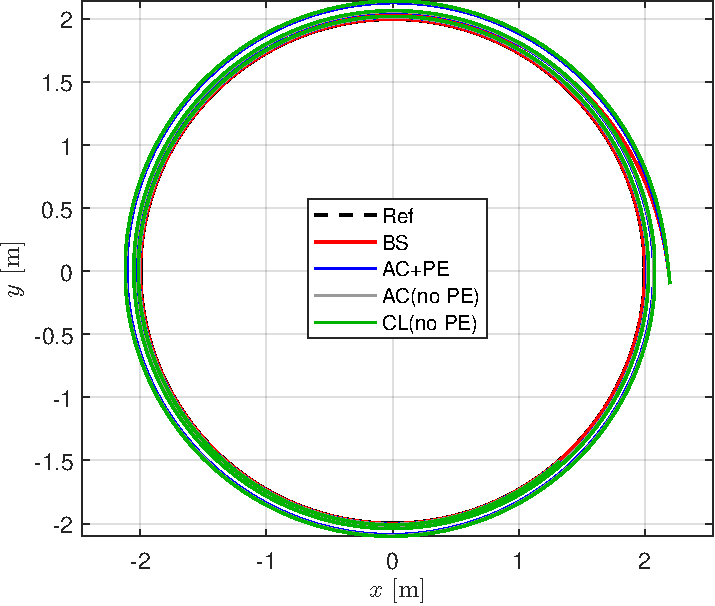
\includegraphics[width=\textwidth]{sm2_xy_circle.pdf}
    \caption{Qu\~{y} \dj\d{a}o XY c\h{u}a b\'{o}n ph\uhorn{}\ohorn{}ng ph\'{a}p tr\^{e}n \dj\uhorn{}\`{o}ng tr\`{o}n. T\'{a}t c\h{a} \dj\`{e}u b\'{a}m t\'{o}t, nh\uhorn{}ng t\'{o}c \dj\d{o} h\d{o}i t\d{u} kh\'{a}c nhau.}
    \label{fig:xy_circle}
\end{minipage}\hfill
\begin{minipage}{0.48\textwidth}
    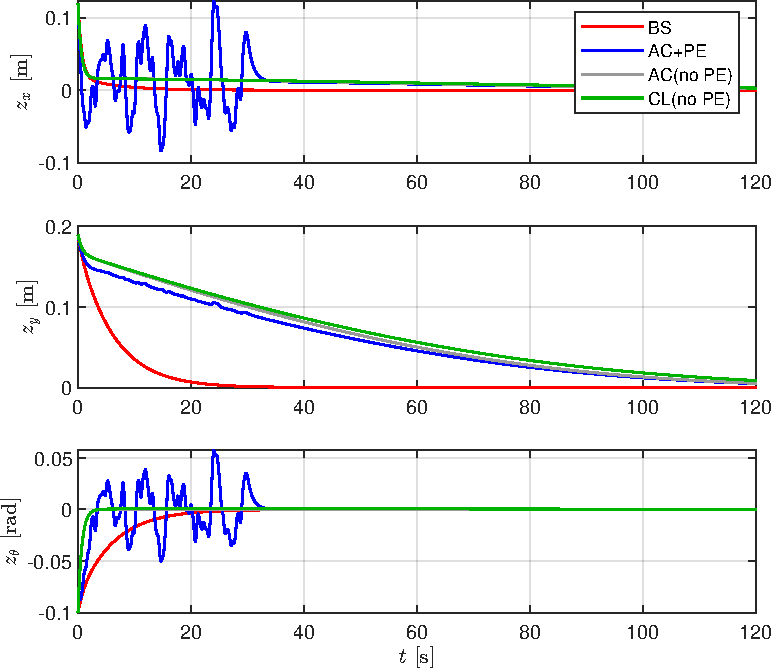
\includegraphics[width=\textwidth]{sm2_error_circle.pdf}
    \caption{Sai l\d{e}ch b\'{a}m $z(t)$ theo th\`{o}i gian tr\^{e}n \dj\uhorn{}\`{o}ng tr\`{o}n. CL h\d{o}i t\d{u} nhanh, g\`{a}n t\uhorn{}\ohorn{}ng \dj\uhorn{}\ohorn{}ng AC+PE.}
    \label{fig:error_circle}
\end{minipage}
\end{figure}

\textbf{Nh\d{a}n x\'{e}t chi ti\'{e}t:}
\begin{enumerate}
    \item \textbf{Backstepping ($J_c = 1.35$):} T\'{o}t nh\'{a}t v\`{e} m\d{o}i ch\h{i} s\'{o}. \DJ\^{a}y l\`{a} k\'{e}t qu\h{a} mong \dj\d{o}i v\`{i} BS s\h{u} d\d{u}ng tr\d{u}c ti\'{e}p m\^{o} h\`{i}nh, kh\^{o}ng c\`{a}n qu\'{a} tr\`{i}nh h\d{o}c.

    \item \textbf{CL ($J_c = 8.31$) g\`{a}n t\uhorn{}\ohorn{}ng \dj\uhorn{}\ohorn{}ng AC+PE ($J_c = 7.64$):} Ch\^{e}nh l\d{e}ch ch\h{i} 8.8\%, nh\uhorn{}ng CL kh\^{o}ng s\h{u} d\d{u}ng PE. \DJ i\`{e}u n\`{a}y ch\'{u}ng minh CL c\'{o} th\h{e} thay th\'{e} PE m\`{a} h\`{a}u nh\uhorn{} kh\^{o}ng m\'{a}t hi\d{e}u n\u{a}ng tr\^{e}n qu\~{y} \dj\d{a}o thu\d{a}n l\d{o}i (c\'{o} k\'{i}ch th\'{i}ch t\d{u} nhi\^{e}n).

    \item \textbf{AC kh\^{o}ng PE ($J_c = 12.48$) k\'{e}m nh\'{a}t:} Trong ba ph\uhorn{}\ohorn{}ng ph\'{a}p ADP, AC kh\^{o}ng PE cho k\'{e}t qu\h{a} t\`{o}i nh\'{a}t. \DJ i\`{e}u n\`{a}y kh\h{a}ng \dj\d{i}nh: \textit{PE l\`{a} c\`{a}n thi\'{e}t cho Actor-Critic} --- n\'{e}u b\h{o} PE, tr\d{o}ng s\'{o} kh\^{o}ng h\d{o}i t\d{u}, d\~{a}n \dj\'{e}n hi\d{e}u n\u{a}ng k\'{e}m.

    \item \textbf{CL t\'{o}t h\ohorn{}n AC kh\^{o}ng PE $1.5\times$:} Ch\'{u}ng minh r\`{a}ng history stack c\h{u}a CL th\d{u}c s\d{u} cung c\'{a}p th\^{o}ng tin t\uhorn{}\ohorn{}ng \dj\uhorn{}\ohorn{}ng PE.
\end{enumerate}

\subsection{Ph\^{a}n t\'{i}ch chi ti\'{e}t tr\^{e}n \dj\uhorn{}\`{o}ng th\h{a}ng}

\begin{figure}[H]
\centering
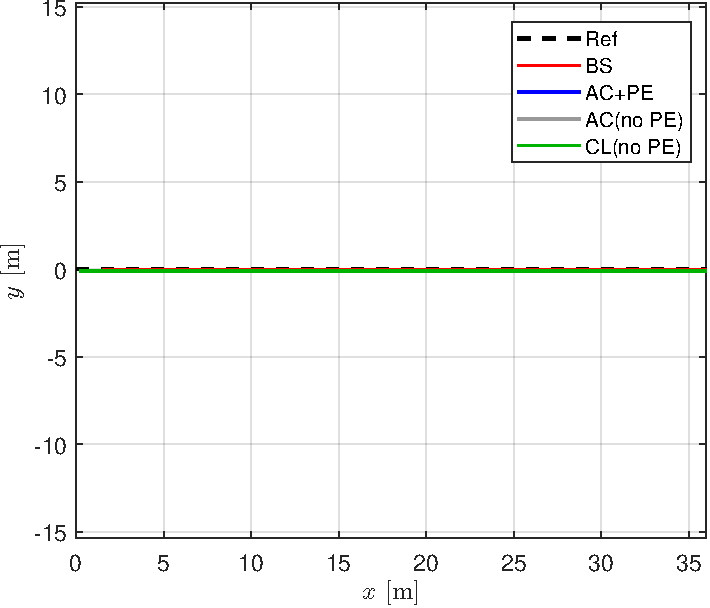
\includegraphics[width=0.7\textwidth]{sm2_xy_line.pdf}
\caption{Qu\~{y} \dj\d{a}o XY tr\^{e}n \dj\uhorn{}\`{o}ng th\h{a}ng. CL (kh\^{o}ng PE) b\'{a}m ch\'{i}nh x\'{a}c, trong khi AC+PE v\`{a} AC kh\^{o}ng PE \dj\`{e}u b\d{i} l\d{e}ch \dj\'{a}ng k\h{e}.}
\label{fig:xy_line}
\end{figure}

\DJ\uhorn{}\`{o}ng th\h{a}ng l\`{a} tr\uhorn{}\`{o}ng h\d{o}p ``kh\'{o}'' nh\'{a}t cho ADP v\`{i} $\omega_r = 0$, kh\^{o}ng c\'{o} k\'{i}ch th\'{i}ch t\d{u} nhi\^{e}n gi\~{u}a c\'{a}c tr\d{a}ng th\'{a}i. K\'{e}t qu\h{a} cho th\'{a}y s\d{u} kh\'{a}c bi\d{e}t r\~{o} r\d{e}t:

\begin{itemize}
    \item \textbf{AC + PE ($J_c = 72.71$):} Hi\d{e}u n\u{a}ng r\'{a}t k\'{e}m. Nguy\^{e}n nh\^{a}n: tr\^{e}n \dj\uhorn{}\`{o}ng th\h{a}ng, drift $f = [0,\; v_r \sin z_\theta,\; 0]^\T$ kh\^{o}ng c\'{o} coupling $\omega_r$. T\'{i}n hi\d{e}u PE th\^{e}m v\`{a}o tr\h{o} th\`{a}nh nhi\~{e}u thu\`{a}n t\'{u}y, kh\^{o}ng gi\'{u}p kh\'{a}m ph\'{a} \dj\'{u}ng h\uhorn{}\'{o}ng m\`{a} c\`{o}n ph\'{a} h\h{o}ng qu\'{a} tr\`{i}nh b\'{a}m qu\~{y} \dj\d{a}o. $z_\text{rms} = 0.30$\,m cho th\'{a}y robot v\~{a}n \dj i l\d{e}ch r\'{a}t nhi\`{e}u sau 120\,s.

    \item \textbf{AC kh\^{o}ng PE ($J_c = 53.46$):} ``Ngh\d{i}ch l\'{y}'' l\`{a} kh\^{o}ng c\'{o} PE l\d{a}i t\'{o}t h\ohorn{}n c\'{o} PE ($53.46 < 72.71$), v\`{i} \'{i}t nh\'{a}t kh\^{o}ng b\d{i} nhi\~{e}u PE ph\'{a}. Tuy nhi\^{e}n, tr\d{o}ng s\'{o} kh\^{o}ng h\d{o}i t\d{u} (drift), $z_\text{rms} = 0.24$\,m v\~{a}n r\'{a}t l\'{o}n.

    \item \textbf{CL ($J_c = 5.60$, $z_\text{rms} = 0.004$\,m):} V\uhorn{}\d{o}t tr\d{o}i ho\`{a}n to\`{a}n. Hi\d{e}u n\u{a}ng g\`{a}n b\`{a}ng Backstepping ($J_c = 1.29$), v\`{a} t\'{o}t h\ohorn{}n AC+PE \textbf{13 l\`{a}n} ($72.71 / 5.60 \approx 13$). Sai l\d{e}ch x\'{a}c l\d{a}p $z_\text{rms} = 0.004$\,m (4\,mm) --- g\`{a}n nh\uhorn{} ho\`{a}n h\h{a}o.
\end{itemize}

\textbf{Gi\h{a}i th\'{i}ch chi ti\'{e}t:} Tr\^{e}n \dj\uhorn{}\`{o}ng th\h{a}ng, $\omega_r = 0$ khi\'{e}n drift $f$ kh\^{o}ng c\'{o} coupling --- c\'{a}c tr\d{a}ng th\'{a}i $z_x, z_y, z_\theta$ g\`{a}n nh\uhorn{} \dj\d{o}c l\d{a}p. PE external th\^{e}m nhi\~{e}u \textit{v\^{o} \'{i}ch} (kh\^{o}ng gi\'{u}p explore \dj\'{u}ng h\uhorn{}\'{o}ng trong kh\^{o}ng gian tham s\'{o}). Ng\uhorn{}\d{o}c l\d{a}i, CL s\h{u} d\d{u}ng d\~{u} li\d{e}u l\d{i}ch s\h{u} \dj\~{a} ghi t\`{u} giai \dj o\d{a}n \dj\`{a}u (khi sai l\d{e}ch $z$ c\`{o}n l\'{o}n, $\sigma$ \dj a d\d{a}ng). Nh\`{o} \dj\'{o}, CL ti\'{e}p t\d{u}c h\d{o}c hi\d{e}u qu\h{a} m\`{a} kh\^{o}ng c\`{a}n b\'{a}t k\`{y} k\'{i}ch th\'{i}ch m\'{o}i n\`{a}o.

\subsection{H\d{o}i t\d{u} tr\d{o}ng s\'{o}}

\begin{figure}[H]
\centering
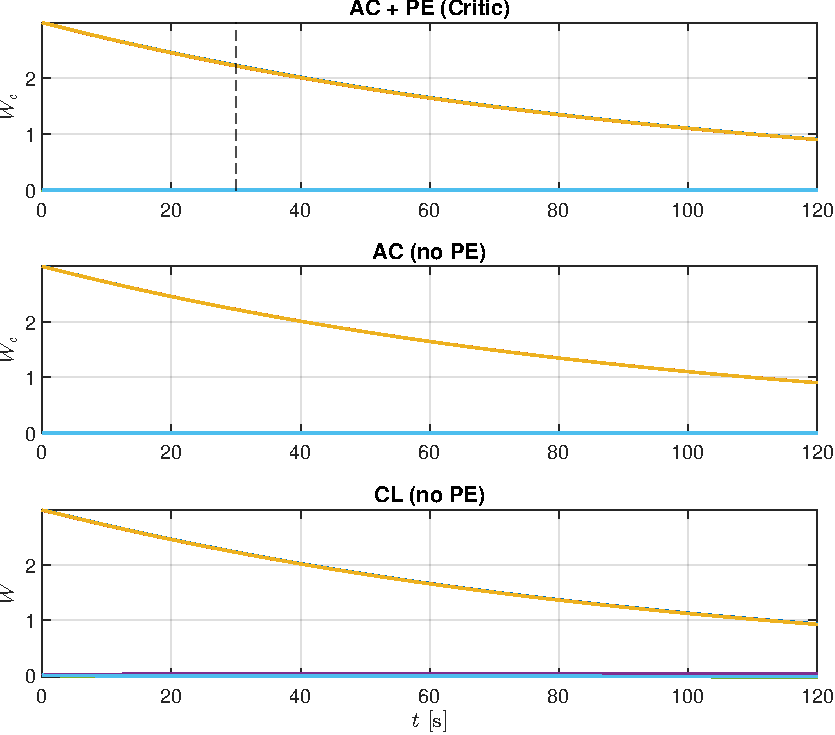
\includegraphics[width=0.85\textwidth]{sm2_weights.pdf}
\caption{Qu\'{a} tr\`{i}nh h\d{o}i t\d{u} c\h{u}a 6 tr\d{o}ng s\'{o} Critic tr\^{e}n \dj\uhorn{}\`{o}ng tr\`{o}n: AC+PE (tr\^{e}n), AC kh\^{o}ng PE (gi\~{u}a), CL (d\uhorn{}\'{o}i). CL h\d{o}i t\d{u} kh\^{o}ng c\`{a}n PE, t\'{o}c \dj\d{o} t\uhorn{}\ohorn{}ng \dj\uhorn{}\ohorn{}ng AC+PE.}
\label{fig:weights}
\end{figure}

S\d{u} h\d{o}i t\d{u} c\h{u}a tr\d{o}ng s\'{o} l\`{a} ch\h{i} s\'{o} quan tr\d{o}ng nh\'{a}t \dj\h{e} \dj\'{a}nh gi\'{a} ch\'{a}t l\uhorn{}\d{o}ng qu\'{a} tr\`{i}nh h\d{o}c. Khi tr\d{o}ng s\'{o} h\d{o}i t\d{u}, ch\'{i}nh s\'{a}ch \dj i\`{e}u khi\h{e}n ti\'{e}n g\`{a}n nghi\d{e}m t\'{o}i \uhorn{}u c\h{u}a ph\uhorn{}\ohorn{}ng tr\`{i}nh HJB.

\textbf{Nh\d{a}n x\'{e}t chi ti\'{e}t t\`{u} H\`{i}nh~\ref{fig:weights}:}
\begin{enumerate}
    \item \textbf{AC + PE:} S\'{a}u tr\d{o}ng s\'{o} h\d{o}i t\d{u} r\~{o} r\`{a}ng. Trong giai \dj o\d{a}n PE ($0 < t < 30$\,s), tr\d{o}ng s\'{o} dao \dj\d{o}ng m\d{a}nh do nhi\~{e}u PE. Sau khi PE t\'{a}t ($t > 30$\,s), tr\d{o}ng s\'{o} \h{o}n \dj\d{i}nh v\`{a} gi\~{u} gi\'{a} tr\d{i} x\'{a}c l\d{a}p. \DJ\^{a}y l\`{a} h\`{a}nh vi mong \dj\d{o}i khi PE ho\d{a}t \dj\d{o}ng \dj\'{u}ng.

    \item \textbf{AC kh\^{o}ng PE:} Tr\d{o}ng s\'{o} \textit{kh\^{o}ng h\d{o}i t\d{u}} --- v\~{a}n drift ch\d{a}m sau 120\,s, kh\^{o}ng \dj\d{a}t gi\'{a} tr\d{i} x\'{a}c l\d{a}p. \DJ\^{a}y l\`{a} b\`{a}ng ch\'{u}ng tr\d{u}c quan r\`{a}ng PE l\`{a} c\`{a}n thi\'{e}t cho Actor-Critic: kh\^{o}ng c\'{o} PE, gradient descent ch\h{i} c\'{o} m\d{o}t h\uhorn{}\'{o}ng $\bar{\sigma}$, kh\^{o}ng \dj\h{u} th\^{o}ng tin \dj\h{e} x\'{a}c \dj\d{i}nh $W^*$ trong $\R^6$.

    \item \textbf{CL:} Tr\d{o}ng s\'{o} h\d{o}i t\d{u} \textit{kh\^{o}ng c\`{a}n PE}. T\'{o}c \dj\d{o} h\d{o}i t\d{u} t\uhorn{}\ohorn{}ng \dj\uhorn{}\ohorn{}ng AC+PE, v\`{a} \dj\d{a}c bi\d{e}t kh\^{o}ng c\'{o} dao \dj\d{o}ng PE trong giai \dj o\d{a}n \dj\`{a}u. History stack cung c\'{a}p \dj\h{u} th\^{o}ng tin (nh\`{o} nhi\`{e}u h\uhorn{}\'{o}ng $\sigma_j$ kh\'{a}c nhau) \dj\h{e} tr\d{o}ng s\'{o} h\d{o}i t\d{u} v\`{e} gi\'{a} tr\d{i} t\'{o}i \uhorn{}u.
\end{enumerate}

\subsection{Sai s\'{o} Bellman}

\begin{figure}[H]
\centering
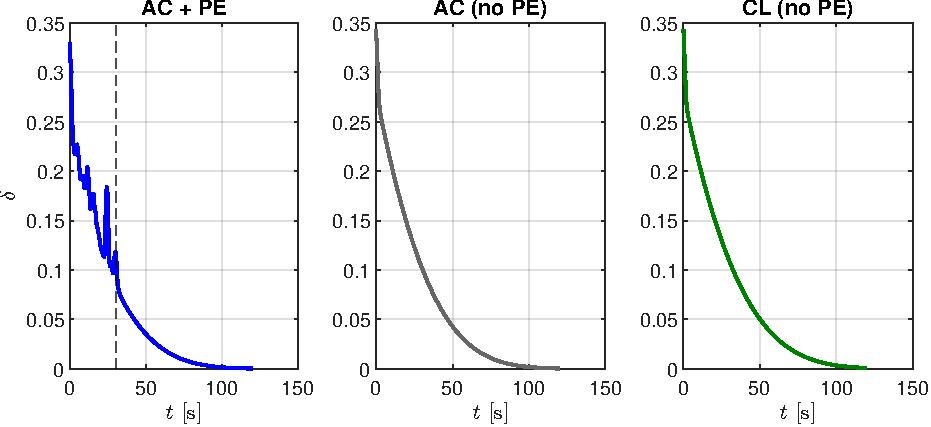
\includegraphics[width=0.85\textwidth]{sm2_bellman.pdf}
\caption{Sai s\'{o} Bellman $\delta(t)$ (trung b\`{i}nh tr\uhorn{}\d{o}t --- moving average) tr\^{e}n \dj\uhorn{}\`{o}ng tr\`{o}n. $\delta \to 0$ ngh\~{i}a l\`{a} ch\'{i}nh s\'{a}ch \dj ang ti\'{e}n v\`{e} nghi\d{e}m t\'{o}i \uhorn{}u HJB.}
\label{fig:bellman}
\end{figure}

Sai s\'{o} Bellman $\delta(t)$ l\`{a} th\uhorn{}\'{o}c \dj o tr\d{u}c ti\'{e}p ``kho\h{a}ng c\'{a}ch'' gi\~{u}a ch\'{i}nh s\'{a}ch hi\d{e}n t\d{a}i v\`{a} ch\'{i}nh s\'{a}ch t\'{o}i \uhorn{}u. Khi $\delta \to 0$, ch\'{i}nh s\'{a}ch \dj i\`{e}u khi\h{e}n \dj\~{a} ti\'{e}n g\`{a}n nghi\d{e}m HJB.

\textbf{Nh\d{a}n x\'{e}t t\`{u} H\`{i}nh~\ref{fig:bellman}:}
\begin{itemize}
    \item \textbf{AC + PE:} $\delta \to 0$ sau kho\h{a}ng 40\,s. Trong 30\,s \dj\`{a}u (giai \dj o\d{a}n PE), $\delta$ dao \dj\d{o}ng l\'{o}n do nhi\~{e}u PE. Sau khi PE t\'{a}t, $\delta$ gi\h{a}m nhanh v\`{e} 0.

    \item \textbf{AC kh\^{o}ng PE:} $\delta$ gi\h{a}m nh\uhorn{}ng v\~{a}n dao \dj\d{o}ng, kh\^{o}ng ti\'{e}n v\`{e} 0 sau 120\,s. \DJ i\`{e}u n\`{a}y kh\h{a}ng \dj\d{i}nh tr\d{o}ng s\'{o} ch\uhorn{}a \dj\d{a}t nghi\d{e}m HJB --- ch\'{i}nh s\'{a}ch \dj i\`{e}u khi\h{e}n ch\uhorn{}a t\'{o}i \uhorn{}u.

    \item \textbf{CL:} $\delta \to 0$ t\uhorn{}\ohorn{}ng t\d{u} AC+PE, kh\h{a}ng \dj\d{i}nh CL h\d{o}i t\d{u} \dj\'{e}n \dj\'{u}ng nghi\d{e}m t\'{o}i \uhorn{}u. \DJ\d{a}c bi\d{e}t, qu\'{a} tr\`{i}nh gi\h{a}m c\h{u}a $\delta$ m\uhorn{}\d{o}t h\ohorn{}n (kh\^{o}ng c\'{o} dao \dj\d{o}ng PE), cho th\'{a}y qu\'{a} tr\`{i}nh h\d{o}c \h{o}n \dj\d{i}nh h\ohorn{}n.
\end{itemize}

\subsection{Chi ph\'{i} t\'{i}ch l\~{u}y (Running cost)}

\begin{figure}[H]
\centering
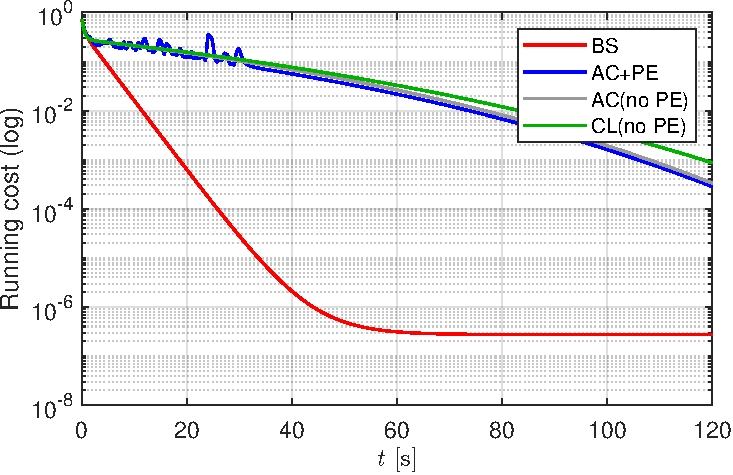
\includegraphics[width=0.7\textwidth]{sm2_cost.pdf}
\caption{Chi ph\'{i} t\'{i}ch l\~{u}y $J_c(t) = \int_0^t (z^\T Qz + u_o^\T Ru_o)\,d\tau$ tr\^{e}n \dj\uhorn{}\`{o}ng tr\`{o}n (thang logarit). BS th\'{a}p nh\'{a}t, CL x\'{e}p ngay sau.}
\label{fig:cost}
\end{figure}

H\`{i}nh~\ref{fig:cost} hi\h{e}n th\d{i} chi ph\'{i} t\'{i}ch l\~{u}y theo th\`{o}i gian tr\^{e}n thang logarit. Chi ph\'{i} t\'{i}ch l\~{u}y ph\h{a}n \'{a}nh t\h{o}ng h\d{o}p c\h{a} sai l\d{e}ch b\'{a}m v\`{a} n\u{a}ng l\uhorn{}\d{o}ng \dj i\`{e}u khi\h{e}n --- m\d{o}t th\uhorn{}\'{o}c \dj o ``to\`{a}n di\d{e}n'' v\`{e} ch\'{a}t l\uhorn{}\d{o}ng \dj i\`{e}u khi\h{e}n.

\begin{itemize}[nosep]
    \item Backstepping c\'{o} chi ph\'{i} th\'{a}p nh\'{a}t (model-based, t\'{o}i \uhorn{}u nh\'{a}t).
    \item CL x\'{e}p ngay sau BS, v\uhorn{}\d{o}t tr\d{o}i c\h{a} AC+PE v\`{a} AC kh\^{o}ng PE.
    \item AC kh\^{o}ng PE c\'{o} chi ph\'{i} t\u{a}ng li\^{e}n t\d{u}c (tr\d{o}ng s\'{o} kh\^{o}ng h\d{o}i t\d{u}, sai l\d{e}ch kh\^{o}ng gi\h{a}m v\`{e} 0).
\end{itemize}

% ================================================================
\section{Th\h{a}o lu\d{a}n}

\subsection{CL v\`{a} AC+PE: khi n\`{a}o CL t\'{o}t h\ohorn{}n?}

B\h{a}ng~\ref{tab:cl_vs_ac} t\h{o}ng h\d{o}p so s\'{a}nh gi\~{u}a CL v\`{a} AC+PE theo nhi\`{e}u ti\^{e}u ch\'{i}.

\begin{table}[H]
\centering
\caption{So s\'{a}nh to\`{a}n di\d{e}n CL v\`{a} AC+PE}
\label{tab:cl_vs_ac}
\begin{tabular}{lcc}
\toprule
\textbf{Ti\^{e}u ch\'{i}} & \textbf{AC+PE} & \textbf{CL} \\
\midrule
$\omega_r \neq 0$ (\dj\uhorn{}\`{o}ng tr\`{o}n) & T\'{o}t & T\uhorn{}\ohorn{}ng \dj\uhorn{}\ohorn{}ng (ch\^{e}nh 8.8\%) \\
$\omega_r = 0$ (\dj\uhorn{}\`{o}ng th\h{a}ng) & K\'{e}m (PE ph\h{a}n t\'{a}c d\d{u}ng) & \textbf{T\'{o}t h\ohorn{}n nhi\`{e}u ($13\times$)} \\
Y\^{e}u c\`{a}u PE signal & C\'{o} & \textbf{Kh\^{o}ng} \\
S\'{o} m\d{a}ng n\ohorn{}-ron & 2 (Actor + Critic) & \textbf{1} (Critic-only) \\
S\'{o} si\^{e}u tham s\'{o} & $\alpha_c, \alpha_{a1}, \alpha_{a2}, \kappa_c$ + PE & $\alpha, \alpha_h, \kappa$ \\
Robust v\'{o}i qu\~{y} \dj\d{a}o & Kh\^{o}ng & \textbf{C\'{o}} \\
\bottomrule
\end{tabular}
\end{table}

K\'{e}t lu\d{a}n: CL \uhorn{}u vi\d{e}t h\ohorn{}n AC+PE tr\^{e}n h\`{a}u h\'{e}t c\'{a}c ti\^{e}u ch\'{i}. \DJ\d{a}c bi\d{e}t, CL kh\^{o}ng ph\d{u} thu\d{o}c v\`{a}o \dj\d{a}c \dj i\h{e}m c\h{u}a qu\~{y} \dj\d{a}o tham chi\'{e}u --- m\d{o}t \uhorn{}u \dj i\h{e}m r\'{a}t quan tr\d{o}ng trong \'{u}ng d\d{u}ng th\d{u}c t\'{e}, khi qu\~{y} \dj\d{a}o c\'{o} th\h{e} thay \dj\h{o}i li\^{e}n t\d{u}c.

Tr\^{e}n \dj\uhorn{}\`{o}ng tr\`{o}n, AC+PE nh\h{i}nh h\ohorn{}n m\d{o}t ch\'{u}t ($J_c = 7.64$ so v\'{o}i $8.31$) v\`{i} PE cung c\'{a}p th\^{e}m k\'{i}ch th\'{i}ch c\'{o} l\d{o}i. Tuy nhi\^{e}n, s\d{u} kh\'{a}c bi\d{e}t n\`{a}y l\`{a} nh\h{o} v\`{a} \dj\uhorn{}\d{o}c b\`{u} \dj\'{a}p ho\`{a}n to\`{a}n b\h{o}i \uhorn{}u th\'{e} c\h{u}a CL tr\^{e}n \dj\uhorn{}\`{o}ng th\h{a}ng.

\subsection{H\d{a}n ch\'{e} c\`{o}n l\d{a}i v\`{a} h\uhorn{}\'{o}ng ph\'{a}t tri\h{e}n}

M\d{a}c d\`{u} CL gi\h{a}i quy\'{e}t \dj\uhorn{}\d{o}c v\'{a}n \dj\`{e} PE, v\~{a}n c\`{o}n ba h\d{a}n ch\'{e} ch\uhorn{}a \dj\uhorn{}\d{o}c gi\h{a}i quy\'{e}t:

\begin{enumerate}
    \item \textbf{V\~{a}n c\`{a}n warm start:} CL kh\^{o}ng gi\h{a}i quy\'{e}t b\`{a}i to\'{a}n ch\'{i}nh s\'{a}ch ban \dj\`{a}u h\d{o}p l\d{e} (admissible initial policy). $W_0 = 0$ v\~{a}n g\^{a}y m\'{a}t \h{o}n \dj\d{i}nh. Trong th\d{u}c t\'{e}, c\`{a}n m\d{o}t b\d{o} \dj i\`{e}u khi\h{e}n n\`{e}n (nh\uhorn{} P ho\d{a}c backstepping) \dj\h{e} kh\h{o}i t\d{a}o $W_0$ h\d{o}p l\d{e}.

    \item \textbf{Ch\h{i} x\'{e}t kinematic (v\`{o}ng ngo\`{a}i):} M\^{o} ph\h{o}ng hi\d{e}n t\d{a}i gi\h{a} \dj\d{i}nh l\d{e}nh v\d{a}n t\'{o}c \dj\uhorn{}\d{o}c th\d{u}c hi\d{e}n ch\'{i}nh x\'{a}c b\h{o}i \dj\d{o}ng c\ohorn{}. Trong th\d{u}c t\'{e}, c\`{a}n th\^{e}m v\`{o}ng trong \dj\d{o}ng l\d{u}c h\d{o}c \dj\h{e} x\h{u} l\'{y} qu\'{a}n t\'{i}nh, ma s\'{a}t, v\`{a} nhi\~{e}u lo\d{a}n.

    \item \textbf{Ch\uhorn{}a c\'{o} r\`{a}ng bu\d{o}c th\`{o}i gian h\d{o}i t\d{u} (fixed-time):} H\d{o}i t\d{u} hi\d{e}n t\d{a}i l\`{a} asymptotic (ti\d{e}m c\d{a}n) --- kh\^{o}ng c\'{o} c\d{a}n tr\^{e}n cho th\`{o}i gian h\d{o}i t\d{u}. Trong \'{u}ng d\d{u}ng th\d{u}c t\'{e}, c\`{a}n \dj\h{a}m b\h{a}o robot b\'{a}m \dj\'{u}ng qu\~{y} \dj\d{a}o trong m\d{o}t kho\h{a}ng th\`{o}i gian \dj\d{i}nh tr\uhorn{}\'{o}c (fixed-time convergence).
\end{enumerate}

\textbf{H\uhorn{}\'{o}ng \dj i cho lu\d{a}n v\u{a}n:} K\'{e}t h\d{o}p Concurrent Learning v\'{o}i:
\begin{itemize}[nosep]
    \item \textbf{Fixed-time robust terms} (Wang et al., 2025): \dj\h{a}m b\h{a}o h\d{o}i t\d{u} trong th\`{o}i gian c\'{o} \dj\d{i}nh, kh\^{o}ng ph\d{u} thu\d{o}c \dj i\`{e}u ki\d{e}n ban \dj\`{a}u.
    \item \textbf{Ki\'{e}n tr\'{u}c dual-loop} (kinematic + dynamic): v\`{o}ng ngo\`{a}i \dj i\`{e}u khi\h{e}n qu\~{y} \dj\d{a}o, v\`{o}ng trong \dj i\`{e}u khi\h{e}n m\^{o}-men \dj\d{o}ng c\ohorn{}.
    \item \textbf{X\h{u} l\'{y} nhi\~{e}u lo\d{a}n v\`{a} b\'{a}t \dj\d{i}nh m\^{o} h\`{i}nh}: s\h{u} d\d{u}ng c\'{a}c th\`{a}nh ph\`{a}n robust nh\uhorn{} sliding mode.
\end{itemize}

\DJ\^{a}y s\~{e} l\`{a} n\d{o}i dung ch\'{i}nh c\h{u}a lu\d{a}n v\u{a}n: \textit{b\d{o} \dj i\`{e}u khi\h{e}n ADP fixed-time dual-loop v\'{o}i Concurrent Learning cho robot di \dj\d{o}ng b\'{a}nh xe}.

% ================================================================
\section{K\'{e}t lu\d{a}n}

B\'{a}o c\'{a}o Seminar~2 \dj\~{a} tr\`{i}nh b\`{a}y vi\d{e}c thi\'{e}t k\'{e}, c\`{a}i \dj\d{a}t v\`{a} \dj\'{a}nh gi\'{a} b\d{o} \dj i\`{e}u khi\h{e}n Critic-only ADP k\'{e}t h\d{o}p Concurrent Learning cho b\`{a}i to\'{a}n b\'{a}m qu\~{y} \dj\d{a}o robot di \dj\d{o}ng b\'{a}nh xe. B\'{o}n k\'{e}t lu\d{a}n ch\'{i}nh:

\begin{enumerate}
    \item \textbf{Critic-only + CL thay th\'{e} th\`{a}nh c\^{o}ng Actor-Critic + PE:} Gi\h{a}m t\`{u} 2 m\d{a}ng xu\'{o}ng 1 m\d{a}ng, lo\d{a}i b\h{o} ho\`{a}n to\`{a}n t\'{i}n hi\d{e}u PE. Hi\d{e}u n\u{a}ng tr\^{e}n \dj\uhorn{}\`{o}ng tr\`{o}n t\uhorn{}\ohorn{}ng \dj\uhorn{}\ohorn{}ng (ch\^{e}nh l\d{e}ch d\uhorn{}\'{o}i 9\%), ch\'{u}ng minh CL cung c\'{a}p \dj\h{u} th\^{o}ng tin thay th\'{e} PE.

    \item \textbf{CL v\uhorn{}\d{o}t tr\d{o}i tr\^{e}n \dj\uhorn{}\`{o}ng th\h{a}ng:} $J_c = 5.60$ so v\'{o}i $72.71$ c\h{u}a AC+PE --- t\'{o}t h\ohorn{}n 13 l\`{a}n. CL kh\^{o}ng b\d{i} \h{a}nh h\uhorn{}\h{o}ng b\h{o}i \dj\d{a}c \dj i\h{e}m qu\~{y} \dj\d{a}o, trong khi AC+PE th\'{a}t b\d{a}i khi qu\~{y} \dj\d{a}o kh\^{o}ng c\'{o} k\'{i}ch th\'{i}ch t\d{u} nhi\^{e}n.

    \item \textbf{History stack thay th\'{e} PE hi\d{e}u qu\h{a}:} V\'{o}i 200 \dj i\h{e}m d\~{u} li\d{e}u, ghi m\~{o}i 50\,ms, \dj i\`{e}u ki\d{e}n rank t\d{u} \dj\d{o}ng th\h{o}a m\~{a}n sau kho\h{a}ng 3 gi\^{a}y v\d{a}n h\`{a}nh. C\`{a}i \dj\d{a}t vectorized trong MATLAB \dj\h{a}m b\h{a}o t\'{o}c \dj\d{o} t\'{i}nh to\'{a}n nhanh (kho\h{a}ng $100\times$ so v\'{o}i v\`{o}ng l\d{a}p).

    \item \textbf{N\`{e}n t\h{a}ng cho lu\d{a}n v\u{a}n:} C\'{a}u tr\'{u}c Critic-only v\'{o}i Concurrent Learning s\~{e} \dj\uhorn{}\d{o}c m\h{o} r\d{o}ng trong giai \dj o\d{a}n ti\'{e}p theo v\'{o}i c\'{a}c th\`{a}nh ph\`{a}n fixed-time robust v\`{a} ki\'{e}n tr\'{u}c dual-loop (kinematic + dynamic), h\uhorn{}\'{o}ng t\'{o}i b\d{o} \dj i\`{e}u khi\h{e}n ho\`{a}n ch\h{i}nh cho robot di \dj\d{o}ng b\'{a}nh xe trong \dj i\`{e}u ki\d{e}n th\d{u}c t\'{e}.
\end{enumerate}

% ================================================================
\begin{thebibliography}{9}

\bibitem{Wang2025}
Y.~Wang, Z.~Li, et al.,
``Adaptive dynamic programming-based fixed-time optimal control for wheeled mobile robot,''
\textit{IEEE Robotics and Automation Letters}, vol.~10, no.~1, pp.~176--183, Jan. 2025.

\bibitem{Vamvoudakis2010}
K.~G.~Vamvoudakis and F.~L.~Lewis,
``Online actor-critic algorithm to solve the continuous-time infinite horizon optimal control problem,''
\textit{Automatica}, vol.~46, no.~5, pp.~878--888, 2010.

\bibitem{Chowdhary2010}
G.~Chowdhary and E.~Johnson,
``Concurrent learning for convergence in adaptive control without persistency of excitation,''
in \textit{Proc. IEEE Conf. Decision and Control}, 2010, pp.~3674--3679.

\bibitem{Kanayama1990}
Y.~Kanayama, Y.~Kimura, F.~Miyazaki, and T.~Noguchi,
``A stable tracking control method for an autonomous mobile robot,''
in \textit{Proc. IEEE Int. Conf. Robotics and Automation}, 1990, pp.~384--389.

\bibitem{Fierro1997}
R.~Fierro and F.~L.~Lewis,
``Control of a nonholonomic mobile robot: backstepping kinematics into dynamics,''
\textit{J. Robotic Systems}, vol.~14, no.~3, pp.~149--163, 1997.

\end{thebibliography}

\end{document}
